%\documentclass[10pt,aspectratio=169]{beamer}
\documentclass[10pt,aspectratio=169,handout]{beamer}
\usepackage{wasysym} 
\usepackage{textcomp}
\usetheme{Boadilla}
\usepackage[utf8]{inputenc}
\usepackage[T1]{fontenc}
\usepackage{lmodern}
\usepackage{lipsum}
\usetheme{default}
\usepackage{listings}
\usepackage{hyperref}
\hypersetup{
	colorlinks=true,
	linkcolor=blue,
	filecolor=magenta,      
	urlcolor=cyan
}
\lstset{language=[90]Fortran,
	basicstyle=\small\ttfamily,
	showtabs=false,
	tabsize=2,      
	keywordstyle=\color{red},
	commentstyle=\color{green},
	morecomment=[l]{!\ }% Comment only with space after !
}

%%%%%%%%%%%%%GTA
%\renewcommand{\(}{\left(}
%\renewcommand{\)}{\right)}
%\renewcommand{\[}{\left[}
%\renewcommand{\]}{\right]}

\newcommand{\calpha}{\alpha^\ast}
\newcommand{\calphas}{\alpha^{\ast2}}
\newcommand{\Kr}[2]{\delta_{#1}^{#2}}

%%%%%%%%%%%%%%%%%%%%


\newcommand{\sqNsotwo}{\sqrt{\dfrac{Ns}{2}}}
\newcommand{\oneoNs}{\dfrac{1}{Ns}}

\let\originalleft\left
\let\originalright\right
\renewcommand{\left}{\mathopen{}\mathclose\bgroup\originalleft}
\renewcommand{\right}{\aftergroup\egroup\originalright}


\newcommand{\vect}[1]{\boldsymbol{#1}}
\renewcommand{\vec}[1]{\vect{#1}}

\makeatletter
\newcommand*\bigcdot{{\color{gray}\mathpalette\bigcdot@{1.}}}
\newcommand*\bigcdot@[2]{\mathbin{\vcenter{\hbox{\scalebox{#2}{$\m@th#1\bullet$}}}}}
\makeatother


\DeclareMathOperator*{\argmax}{argmax}
\DeclareMathOperator*{\argmin}{argmin}
\def\rme{{\rm {e}}}
\def\rmi{{\rm {i}}}
\renewcommand{\d}{{\rm {d}}}
\def\dt{{\rm {d}}t}
\def\dddt{\dfrac{\d}{\dt}}
\def\ddt{\frac{\d}{\dt}}

% \newcommand{\sgn}{\mathop{\mathrm{sgn}}}

\newcommand{\diag}{\mathrm{diag}}


\newcommand{\idhat}{\hat{\mathds{1}}}
\newcommand{\id}{\mathds{1}}
\newcommand{\idres}{\id_\mathrm{res}}
\newcommand{\idsys}{\id_\mathrm{sys}}

\newcommand{\trfrak}{\mathfrak{Tr}}
\def\tr{{\rm{Tr}}}
\newcommand{\abss}[1]{\left|#1\right|^2}
\newcommand{\mean}[1]{\left\langle #1 \right\rangle}
\newcommand{\expect}[1]{\mathbb{E}\left[ #1\right]}

%%%%%%%%%%%%%%%%%%% units
\newcommand{\micron}{\rm{\si{\micro\meter}}}


%%%%%%%%%%%%%%%%%%% Greek letters

\newcommand{\alphatil}{{\Tilde{\alpha}}}
\newcommand{\ass}{\alpha_{\mathrm{SS}}}
\newcommand{\alphass}{\alpha_\mathrm{SS}}
\newcommand{\alphahat}{\hat{\alpha}}
\newcommand{\betahat}{\hat{\beta}}
\newcommand{\betatil}{{\Tilde{\beta}}}
% \newcommand{\betatil}{\Tilde{\beta}}

\newcommand{\delhat}{\hat{\delta}}
\newcommand{\ddelhat}{\hat{\delta}^\dagger}

\newcommand{\Jhat}{\hat{J}}

\newcommand{\Lammat}{\boldsymbol{\Lambda}}

\newcommand{\lambdown}{\lambda^{\downarrow}}

\newcommand{\rhoh}{\hat{\rho}}

\newcommand{\rhohat}{\hat{\rho}}
\newcommand{\rhotil}{\tilde{\rho}}
\newcommand{\rhoss}{\rhohat_{\mathrm{SS}}}

\newcommand{\phihat}{\hat{\phi}}
\newcommand{\phidot}{\Dot{\phi}}
\newcommand{\phimat}{\vec{\Phi}}

\newcommand{\Pihat}{\hat{\Pi}}
\newcommand{\pihat}{\hat{\pi}}
\newcommand{\piit}{\mathit{\Pi}}
\newcommand{\piithat}{\hat{\piit}}

\newcommand{\psitilde}{\widetilde{\ket{\psi}}}

\newcommand{\epsvec}{\vec{\epsilon}}

\newcommand{\Obold}{\mathbf{\Omega}}

\newcommand{\Gammatil}{\Tilde{\Gamma}}

\newcommand{\sigmam}{\hat{\sigma}^{-}}
\newcommand{\sigmap}{\hat{\sigma}^{+}}
\newcommand{\sigmax}{\hat{\sigma}^{x}}
\newcommand{\sigmay}{\hat{\sigma}^{y}}
\newcommand{\sigmaz}{\hat{\sigma}^{z}}
\newcommand{\sigmamz}{\hat{\sigma}^{-z}}
\newcommand{\sigmamx}{\hat{\sigma}^{-x}}

\newcommand{\ssp}{\hat{\sigma}^+}
\newcommand{\ssm}{\hat{\sigma}^-}
\newcommand{\ssx}{\hat{\sigma}^x}
\newcommand{\ssy}{\hat{\sigma}^y}
\newcommand{\ssz}{\hat{\sigma}^z}
\newcommand{\ssa}{\hat{\sigma}^\alpha}
\newcommand{\sssz}{\hat{\sigma}^z}
\newcommand{\sigbold}{\bm{\sigma}}

\newcommand{\sigmahat}{\hat{\sigma}}

%%%%%%%%%%%%%%%% abbreviations
\newcommand{\schr}{Schr\"{o}dinger}
\newcommand{\kg}{{\mathrm{KG}}}

\newcommand{\hc}{\mathrm{H.c.}}
%\newcommand{\pv}{\mathrm{p.v.}}

\newcommand{\LP}{\mathrm{LP}}
\newcommand{\UP}{\mathrm{UP}}

%%%%%%%%%%%%%%%% Latin letters


\newcommand{\aaa}{\hat{a}}
\newcommand{\daaa}{\hat{a}^\dagger}
\newcommand{\daaas}{\hat{a}^{\dagger 2}}
\newcommand{\aaas}{\aaa^{2}}

\newcommand{\Ahat}{\hat{A}}
\newcommand{\dAhat}{\Ahat^{\dagger}}
\newcommand{\Atil}{\hat{\tilde{A}}}
\newcommand{\dAtil}{\hat{\tilde{A}}^\dagger}


\newcommand{\Avec}{\vec{A}}
\newcommand{\Avechat}{\hat{\bm{A}}}
\newcommand{\acal}{\mathcal{A}}

\newcommand{\bbb}{\hat{b}}
\newcommand{\dbbb}{\hat{b}^\dagger}
\newcommand{\bbbs}{\bbb^{2}}
\newcommand{\dbbbs}{\bbb^{\dagger 2}}

\newcommand{\BS}{\widehat{\mathrm{BS}}}

\newcommand{\bvec}{\vec{b}}

\newcommand{\Bvec}{\vec{B}}
\newcommand{\Bvechat}{\hat{\bm{B}}}

\newcommand{\Bhat}{\hat{B}}

\newcommand{\cvec}{\vec{c}}
% \newcommand{\ccal}{\mathcal{C}}
\newcommand{\ccc}{\hat{c}}
\newcommand{\dccc}{\hat{c}^\dagger}

\newcommand{\ccal}{\mathcal{C}}

\newcommand{\dcal}{\mathcal{D}}

\newcommand{\dvec}{\vec{d}}

\newcommand{\Ehat}{\hat{E}}
\newcommand{\Evec}{\vec{E}}
\newcommand{\evec}{\vec{e}}
\newcommand{\Evechat}{\hat{\bm{E}}}
\newcommand{\ecal}{\mathcal{E}}



\newcommand{\Fbold}{\mathbf{F}}

\newcommand{\fhat}{\hat{f}}
\newcommand{\fcal}{\mathcal{F}}
\newcommand{\gcal}{\mathcal{G}}
\newcommand{\Gmat}{\boldsymbol{\mathrm{G}}}

% \newcommand{\Ehat}{\hat{E}}
\newcommand{\ecalf}{\ecal^{F}}

\newcommand{\ecalu}{\ecal^{U}}
\newcommand{\fcalu}{\fcal^{U}}
\newcommand{\czu}{\ccal_{\ztil}^{U}}

\newcommand{\ecaluc}{\ecal^{U*}}
\newcommand{\fcaluc}{\fcal^{U*}}
\newcommand{\czuc}{\ccal_{\ztil}^{U*}}

\newcommand{\ecald}{\ecal^{D}}
\newcommand{\fcald}{\fcal^{D}}
\newcommand{\czd}{\ccal_{\ztil}^{D}}

\newcommand{\ecaldc}{\ecal^{D*}}
\newcommand{\fcaldc}{\fcal^{D*}}
\newcommand{\czdc}{\ccal_{\ztil}^{D*}}

\newcommand{\ecali}{\ecal^{I}}
\newcommand{\fcali}{\fcal^{I}}
\newcommand{\czi}{\ccal_{\ztil}^{I}}

\newcommand{\ecalic}{\ecal^{I*}}
\newcommand{\fcalic}{\fcal^{I*}}
\newcommand{\czic}{\ccal_{\ztil}^{I*}}


\newcommand{\hcal}{\mathcal{H}}
\newcommand{\hh}{\hat{H}}
\newcommand{\heff}{\hat{H}_\text{eff}}

\newcommand{\Hhat}{\hat{H}}
\newcommand{\hhat}{\hat{h}}
\newcommand{\htil}{\tilde{H}}

\newcommand{\Khat}{\hat{K}}
\newcommand{\kvec}{{\vec{k}}}


\newcommand{\lio}{\mathcal{L}}
\newcommand{\liou}{\mathcal{L}}
\newcommand{\Liou}{\liou}

\newcommand{\lioeff}{\mathcal{L}_\text{eff}}

\newcommand{\lcal}{\mathcal{L}}
\newcommand{\Lhat}{\hat{L}}
\newcommand{\Ltil}{\tilde{L}}
\newcommand{\Lcal}{\mathcal{L}}

\newcommand{\mev}{\mathrm{meV}}


\newcommand{\mcal}{\mathcal{M}}

\newcommand{\mvec}{{\vec{m}}}
\newcommand{\nsys}{{N_\mathrm{sys}}}
\newcommand{\nres}{{N_\mathrm{res}}}

\newcommand{\ncal}{\mathcal{N}}

\newcommand{\nvec}{{\vec{n}}}

\newcommand{\ohat}{\hat{O}}
\newcommand{\otil}{\tilde{O}}
\newcommand{\ovec}{{\vec{0}}}
\newcommand{\ocal}{\mathcal{O}}

\newcommand{\Ohat}{\hat{O}}

\newcommand{\phat}{\hat{p}}
\newcommand{\pvec}{\vec{p}}
\newcommand{\pcal}{\mathcal{P}}
\newcommand{\pscr}{{\mathscr{P}}}

\newcommand{\qdot}{\dot{q}}
\newcommand{\qhat}{\hat{q}}
\newcommand{\qvec}{\vec{q}}
\newcommand{\qcal}{\mathcal{Q}}
\newcommand{\Rhat}{\hat{R}}
\newcommand{\Rtil}{\tilde{R}}

\newcommand{\R}{\mathbb{R}}

\newcommand{\rvec}{\vec{r}}
\newcommand{\res}{\mathrm{res}}

\newcommand{\rf}{{\mathrm{RF}}}

\newcommand{\Shat}{\hat{S}}
\newcommand{\shat}{\hat{s}}
\newcommand{\svec}{\hat{\vec{\sigma}}}
\newcommand{\sys}{\mathrm{sys}}

\newcommand{\Svec}{\vec{S}}
\newcommand{\Stil}{\tilde{S}}
\newcommand{\Sbold}{\mathbf{S}}
\newcommand{\scal}{\mathcal{S}}

\newcommand{\tcal}{\mathcal{T}}

\newcommand{\Uhat}{\uhat}
\newcommand{\uhat}{\hat{U}}
\newcommand{\udag}{\hat{U}^\dagger}
\newcommand{\Umat}{\boldsymbol{\mathrm{U}}}
\newcommand{\uvec}{\vec{u}}

\newcommand{\ua}{u^{(a)}}
\newcommand{\uac}{u^{(a)*}}
\newcommand{\uab}{u^{(ab)}}
\newcommand{\uabc}{u^{(ab)*}}
\newcommand{\ub}{u^{(b)}}
\newcommand{\ubc}{u^{(b)*}}




\newcommand{\delhata}{\hat{\delta}^{(a)}}
\newcommand{\delhatb}{\hat{\delta}^{(b)}}

\newcommand{\ddelhata}{\hat{\delta}^{(a)\dagger}}
\newcommand{\ddelhatb}{\hat{\delta}^{(b)\dagger}}

\newcommand{\wvec}{\vec{w}}

\newcommand{\xhat}{\hat{x}}

\newcommand{\xvec}{\vec{x}}
\newcommand{\xmu}{x^{\mu}}
\newcommand{\xpmu}{x^{\prime\mu}}
\newcommand{\xnu}{x^{\nu}}
\newcommand{\xpnu}{x^{\prime\nu}}

\newcommand{\rmx}{\mathrm{x}}
\newcommand{\xvecrm}{\vec{\mathrm{x}}}
\newcommand{\rmxvec}{\xvecrm}
\newcommand{\Xvec}{\vec{X}}
\newcommand{\xcal}{\mathcal{X}}

\newcommand{\xtil}{{\Tilde{x}}}

\newcommand{\yvec}{\vec{y}}
\newcommand{\ycal}{\mathcal{Y}}
\newcommand{\ytil}{{\Tilde{y}}}

\newcommand{\Vhat}{\hat{V}}
\newcommand{\ztil}{{\Tilde{z}}}
\newcommand{\z}{\mathbb{Z}}
\newcommand{\zerovec}{\vec{0}}
\newcommand{\zvec}{{\vec{z}}}

\newcommand{\zcal}{\mathcal{Z}}
% \renewcommand{\ket}[1]{|#1\rangle}

\newcommand{\pmx}[1]{\begin{pmatrix}
		#1
\end{pmatrix}}


\newcommand{\bea}{\begin{equation*}\begin{aligned}}
		\newcommand{\eea}{\end{aligned}\end{equation*}}
\newcommand{\be}{\begin{equation*}}
	\newcommand{\ee}{\end{equation*}}

\newcommand{\redtext}[1]{\textcolor{red}{#1}}

\begin{document}
\author{Zejian Li \\(li.zejian@ictp.it)}
\title{Lecture 1-1: Nonlinear Regression}
\subtitle{with least-squares fitting}
%\logo{}
%\institute{}
\date{18 Oct. 2024}
%\subject{}
%\setbeamercovered{transparent}
%\setbeamertemplate{navigation symbols}{}


% ----------------------------------------------------------------
\begin{frame}[plain]
	\maketitle
\end{frame}


% ----------------------------------------------------------------
\section{Introduction}

\begin{frame}
	\frametitle{Last lecture: {\color{blue} linear} least-squares fitting}
	The process of constructing a parametrized {\color{blue}linear} function $f(\vec{x}; \vec{\beta})$ that has the best fit to a series of data points $\{(\vec{x}_i,y_i)\}_i$. \\ \pause
	
	\vspace{-0.5cm}
	\begin{columns}[t]
	\column{0.5\textwidth}
		\begin{itemize}[<+->]
		\item {\color{blue} Linear} model:
		\bea
		f(\vec{x};\vec{\beta}) &= \vec{x}\vec{\beta}\,,\quad \vec{x}\in\mathbb{R}^{1\times D}\,,\vec{\beta}\in\mathbb{R}^{D\times 1}\,,\\
		y_i &= f(\vec{x})_i + \varepsilon_i\,,\quad \varepsilon\sim\ncal(0,\sigma^2\mathbb{I})\,.
		\eea
		\end{itemize}
	\vspace{-0.3cm}
		\begin{figure}
			\centering
			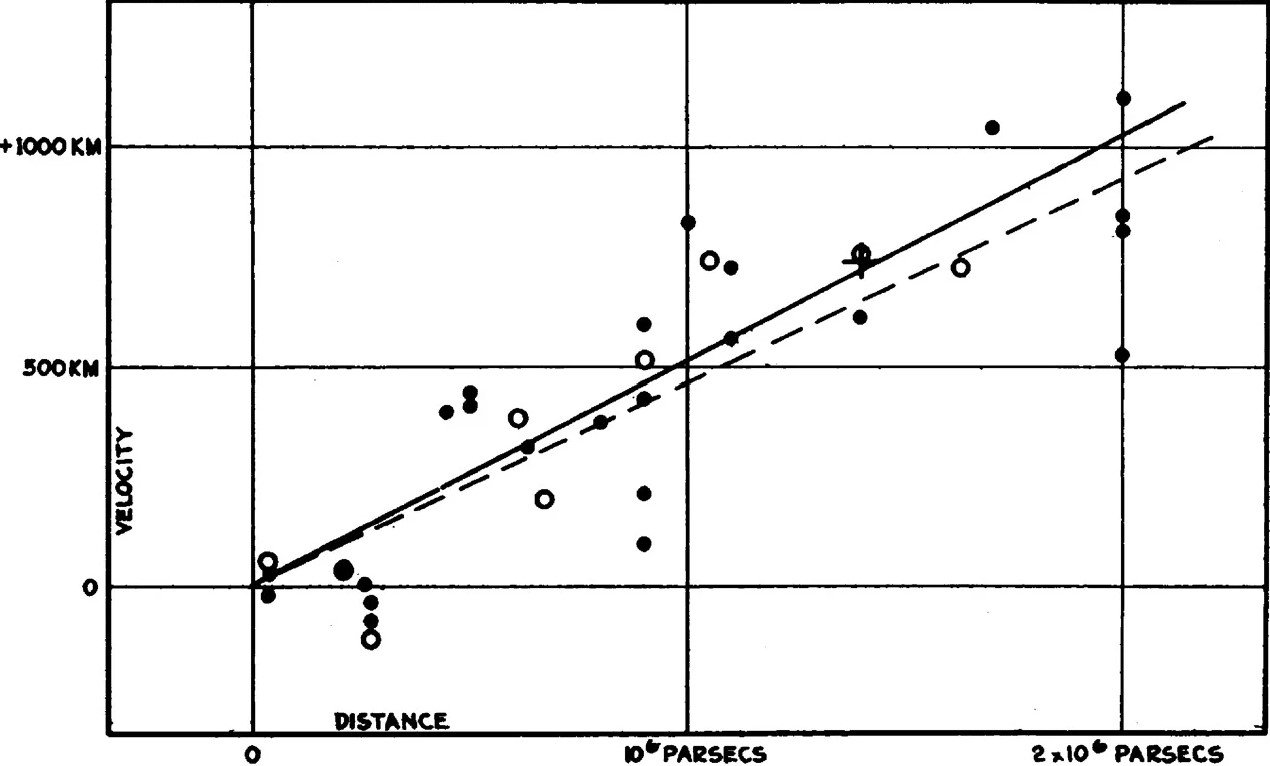
\includegraphics[width=0.8\textwidth]{fig/hubble.jpg}
		\end{figure}%

		\column{0.5\textwidth}
		\begin{itemize}[<+->]
			
			\item Best fit:
			\bea
			\hat{\vec{\beta}} = (\mathbf{X}^T\mathbf{X})^{-1}\mathbf{X}^T\vec{y}\,,
			\eea
			where
			\bea
			\mathbf{X} \equiv \begin{bmatrix}
				\vec{x}_1 \\
				\vdots \\
				\vec{x}_N
			\end{bmatrix}\,,\quad 
			\vec{y} \equiv  \begin{bmatrix}
				y_1\\
				\vdots \\
				y_N
			\end{bmatrix}\,.
			\eea
			
			\item Error estimation
			\bea
			\sigmahat^2 &= \sum_{i = 1}^N\dfrac{[y_i-f(\vec{x}_i;\hat{\vec{\beta}})]^2}{N - D}\,,\\
			\widehat{\mathrm{Var}}(\hat{\vec{\beta}}) &= \sigmahat^2  (\mathbf{X}^T\mathbf{X})^{-1}\,.
			\eea
		\end{itemize}
		\end{columns}

\end{frame}



\begin{frame}{Today: {\color{red} nonlinear} least-squares fitting}
	The process of constructing a parametrized {\color{red}nonlinear} function $f(\vec{x}; \vec{\beta})$ that has the best fit to a series of data points $\{(\vec{x}_i,y_i)\}_i$. \pause
	\begin{columns}
		\column{0.5\textwidth}
			\begin{itemize}[<+->]
				\item {\color{red} Nonlinear} model: $f(\vec{x}; \vec{\beta})$ some generic nonlinear function with parameters $\vec{\beta}$.\\
				For example...
				\vspace{0.1cm}
				\begin{itemize}
					\item $ f(t;\beta_1,\beta_2) = \beta_1\rme^{-\beta_2 t} $ (exponential decay).
					\vspace{0.1cm}
					\item $ B_\lambda(\lambda; T) = \dfrac{2h c^2}{\lambda^5}\dfrac{1}{\rme^{hc/(\lambda k_BT)}-1} $ (Plank's law for blackbody radiation).
				\end{itemize}
				\item Assumption on errors (same as before): \bea
				y_i = f(\vec{x}_i) + \varepsilon_i\,,\quad
				\varepsilon\sim\ncal(0,\sigma^2\mathbb{I})\,.\eea
				 \item Objective: minimize sum of squared residuals:
				 \bea
				 	S_{\mathrm{res}} = \sum_i[y_i - f(\vec{x}_i)]^2\,.
				\eea
			\end{itemize}
		\column{0.45\textwidth}
		\vspace{-0.2cm}
		\onslide<1->\begin{figure}
			\centering
			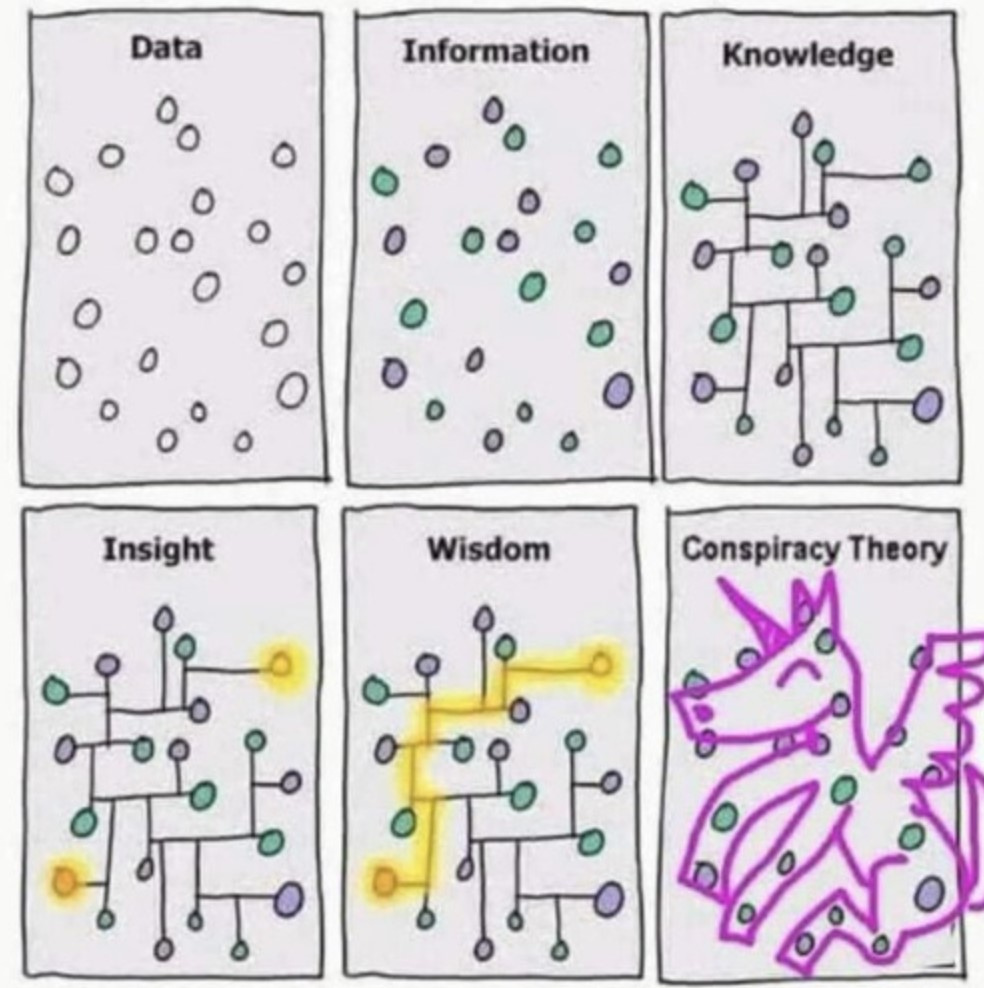
\includegraphics[width=0.8\textwidth]{fig/overfit}
		\end{figure}%
	\begin{center}
		\vspace{-0.2cm}
	Always be careful with overfitting...
	\end{center}

	\end{columns}
\end{frame}

\begin{frame}{Nonlinear least-squares fitting}
We now try to minimize $S_\mathrm{res}$ in the same way as before:
	\bea
		S_{\mathrm{res}}(\vec{\beta}) = \sum_i[y_i - f(\vec{x}_i;\vec{\beta})]^2\,.
	\eea
	\vspace{-0.5cm}\pause
	\begin{itemize}[<+->]
	\item and compute the partial derivatives...
	\bea
		\dfrac{\partial S_\mathrm{res}}{\partial \beta_j} = 2\sum_i[ f(\vec{x}_i;\vec{\beta}) - y_i ]\dfrac{\partial f(\vec{x}_i;\vec{\beta})}{\partial\beta_j} = \text{something nonlinear in } \vec{\beta} \text{ in general \frownie{}}
	\eea
	\item There is no closed-form solution so we have to proceed iteratively: starting from an initial guess for $\vec{\beta}$ and improve the guess little by little.
	\item Since we know how to solve linear least-squares, let's linearize $f$ around the current value of $\vec{\beta}$:
	\bea
		f(\vec{x};\vec{\beta}+\Delta\vec{\beta}) \simeq f(\vec{x};\vec{\beta}) + \sum_j \dfrac{\partial f(\vec{x};\vec{\beta})}{\partial\beta_j} \Delta\beta_j\,,\quad \text{for small } \Delta\vec{\beta}\,.
	\eea
	\item The linearized problem becomes finding $\Delta\vec{\beta}$ such that
	\bea
		\sum_i\left[ f(\vec{x}_i;\vec{\beta}) + \sum_j \dfrac{\partial f(\vec{x}_i;\vec{\beta})}{\partial\beta_j} \Delta\beta_j - y_i \right]\dfrac{\partial f(\vec{x}_i;\vec{\beta})}{\partial\beta_j} = 0\,.
	\eea
	
\end{itemize}
\end{frame}

\begin{frame}{Nonlinear least-squares fitting}
	\begin{itemize}[<+->]
		\item The linearized problem becomes finding $\Delta\vec{\beta}$ such that
		\bea
		\sum_i\left[ f(\vec{x}_i;\vec{\beta}) + \sum_j \dfrac{\partial f(\vec{x}_i;\vec{\beta})}{\partial\beta_j} \Delta\beta_j - y_i \right]\dfrac{\partial f(\vec{x}_i;\vec{\beta})}{\partial\beta_j} = 0\,.
		\eea
		\item Let's clean up this equation a bit by defining:
		\vspace{-0.2cm}
		\bea
			r_i \equiv  y_i - f(\vec{x}_i;\vec{\beta})\,, \quad J_{ij} = \dfrac{\partial f(\vec{x}_i;\vec{\beta})}{\partial\beta_j}\,,
		\eea
		\vspace{-0.5cm}
		\item and after rearranging the terms, we get
		\bea
			\mathbf{J}^T \mathbf{J}\Delta\vec{\beta} = \mathbf{J}^T \vec{r}\quad\longrightarrow \quad \Delta\vec{\beta} = (\mathbf{J}^T \mathbf{J})^{-1}\mathbf{J}^T \vec{r}\,.
		\eea
		This is a linear system that we know how to solve! \smiley{}\\
		 (Note that the \textit{Jacobian} matrix $\mathbf{J}$ plays the role of $\mathbf{X}$ in the linear case.)
		\item Since the linearization of $f(\vec{x};\vec{\beta})$ only makes sense locally around $\vec{\beta}$, we move $\vec{\beta}$ by a \textbf{small} step in the direction of $\Delta\vec{\beta}$ for our next guess:
		\bea
			\vec{\beta} \leftarrow \vec{\beta} + \alpha \Delta\vec{\beta}\,,
		\eea
		for some small $\alpha\in(0,1)$ (for example a constant $\alpha=0.1$).
		\item We then iterate using the new guess until convergence.
	\end{itemize}

\end{frame}

\begin{frame}{Nonlinear least-squares fitting: summary}
	\begin{columns}
		\column{0.65\textwidth}
		\begin{block}{Algorithm: damped Gauss-Newton method}
			\textbf{Input}: dataset $\{(\vec{x}_i,y_i)\}_i$, model function $f(\vec{x};\vec{\beta})$, small step length $\alpha$, small threshold $\epsilon$ and a large \texttt{maxIter}. \\
			\pause
			\begin{enumerate}
				\item Set $\vec{\beta}$ to some initial guess $\vec{\beta}^{(0)}$.\pause
				\item \texttt{DO k = 1, maxIter}
				\begin{itemize}[<+->]
					\pause\item Construct the vector $\vec{r}$ of residuals $r_i \equiv  y_i - f(\vec{x}_i;\vec{\beta})$.
					\item Construct the Jacobian matrix $J_{ij} = \dfrac{\partial f(\vec{x}_i;\vec{\beta})}{\partial\beta_j}$.
					\item Find the descent direction $\Delta\vec{\beta} = (\mathbf{J}^T \mathbf{J})^{-1}\mathbf{J}^T \vec{r}$.
					\vspace{0.2cm}
					\item \texttt{IF}~ $||\Delta\vec{\beta}||_2^2 \equiv \sum_j \Delta\beta_j^2 <= \epsilon$~ \texttt{EXIT}.
					\vspace{0.2cm}
					\item Update fit parameters with $\vec{\beta}\leftarrow\vec{\beta}+\alpha\Delta\vec{\beta}$.
				\end{itemize}
				\onslide<3->\texttt{END DO}
			\end{enumerate}
			\pause
			\textbf{Output}: Best fit parameters $\hat{\vec{\beta}}$.
		\end{block}
			\column{0.3\textwidth}\pause
		\begin{figure}
			\centering
			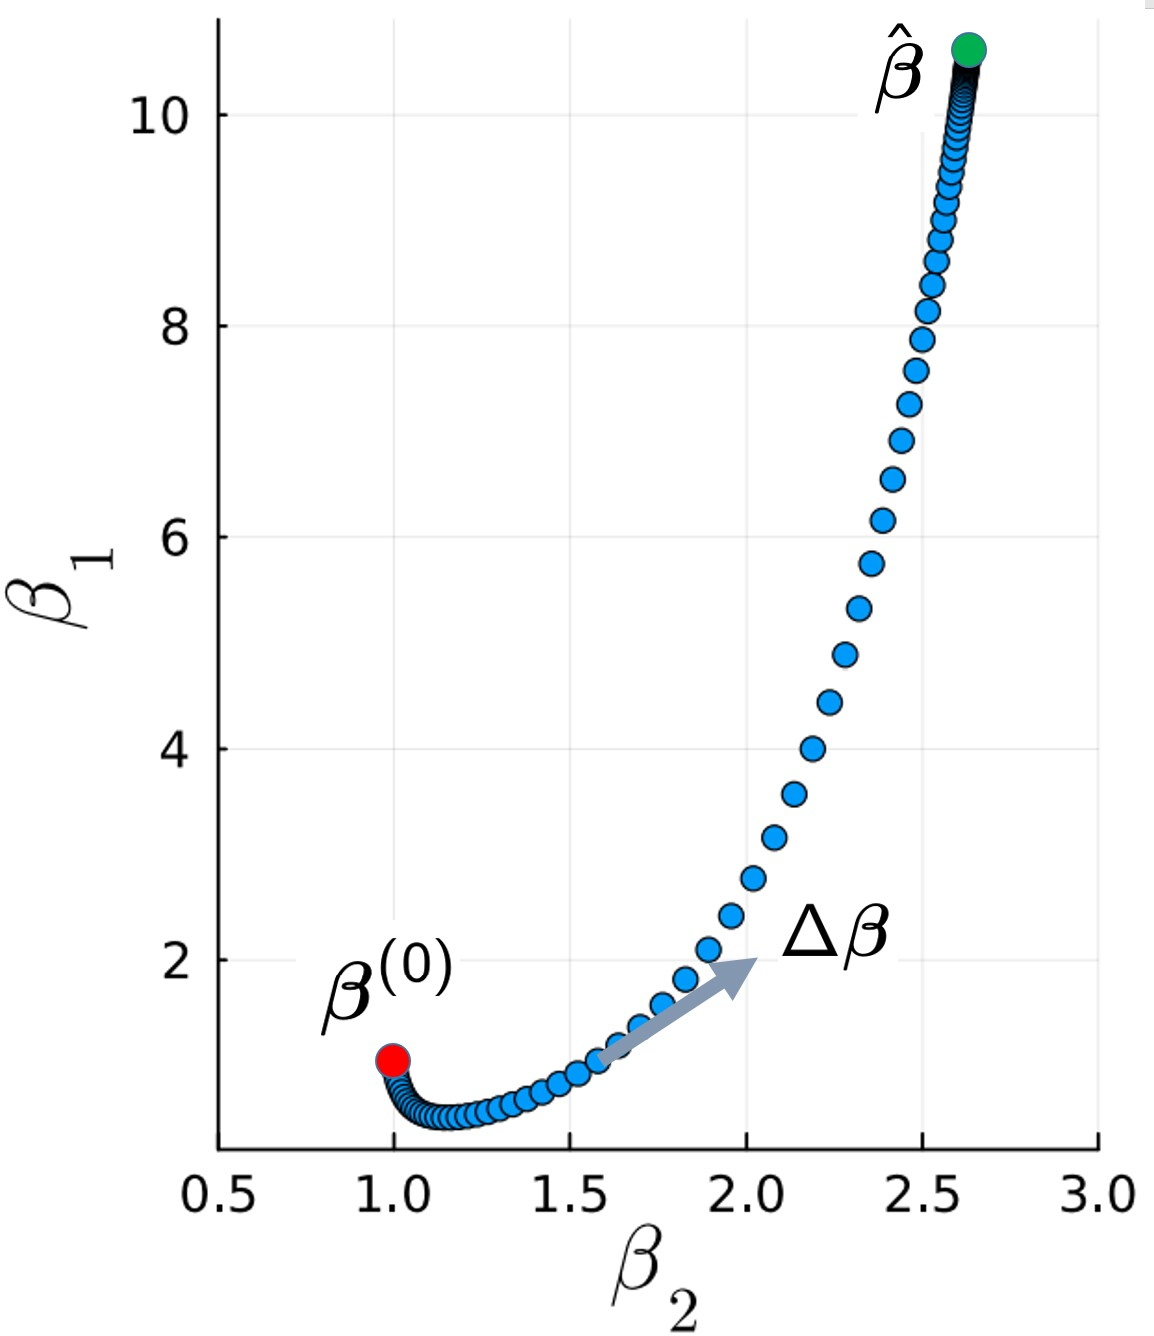
\includegraphics[width=\textwidth]{fig/beta_plot}
		\end{figure}
 
	\end{columns}
\end{frame}


\begin{frame}{Error estimation}
	\begin{itemize}[<+->]	
		\item Estimator for the variance $\sigma^2$ of the error $\varepsilon_i = y_i - f(x_i)$:
		\bea
		\sigmahat^2 = \sum_{i = 1}^N\dfrac{\varepsilon_i^2}{N-D} =\dfrac{S_\mathrm{res}(\hat{\vec{\beta}})}{N-D} \,.
		\eea
		\item Standard errors (SE) for the fit parameters:
		\bea
		\widehat{\mathrm{Var}}(\hat{\vec{\beta}}) = \sigmahat^2  \left[\mathbf{J(\hat{\vec{\beta}})}^T\mathbf{J(\hat{\vec{\beta}})}\right]^{-1}\,,\quad \widehat{\mathrm{SE}}(\betahat_i) = \sqrt{\widehat{\mathrm{Var}}(\hat{\vec{\beta}})_{i,i}}\,.
		\eea
			 (Again, note that the \textit{Jacobian} matrix $\mathbf{J}$ plays the role of $\mathbf{X}$ in the linear case.)
		\item What about $R^2$?\pause \\
		  ...It's not valid for nonlinear least-squares (even though some still use it).\pause \\
		See, for example, ``\href{https://pmc.ncbi.nlm.nih.gov/articles/PMC2892436/}{An evaluation of $R^2$ as an inadequate measure for nonlinear models in pharmacological and biochemical research: a Monte Carlo approach}''.
		
		
	\end{itemize}

\end{frame}


\begin{frame}{Assignment: estimate the sun surface temperature}
	Almost all the radiation that enters the Earth's atmosphere comes from the Sun, which originates in thermonuclear reactions in the core of the Sun. Most of the light emitted by the sun is characteristic of a blackbody radiator described by the Plank's law:
	\vspace{-0.2cm}
	\bea
		 B_\lambda(\lambda; T) = \dfrac{2h c^2}{\lambda^5}\dfrac{1}{\rme^{hc/(\lambda k_BT)}-1}\,,
	\eea
	where $T$ is the temperature and $B_\lambda$ denotes the spectral energy density (intensity per unit wavelength) of the radiation. In the text file \texttt{sun\_data.txt} you can find the data for $B_\lambda$ (in $\mathrm{W}\cdot\mathrm{m}^{-2}\cdot\mathrm{nm}^{-1}$) as a function of $\lambda$ (in microns) measured from sunlight.
	 \textbf{Write a Fortran program to perform a nonlinear fit of the data and estimate the surface temperature of the sun.}\\ \pause
	\begin{itemize}[<+->]
		\item Perform the fit with the nonlinear model $ B(\lambda;\beta_1,\beta_2) = \dfrac{\beta_1}{\lambda^5( \rme^{\beta_2/\lambda}-1)}$ 
		\item Use the damped Gauss-Newton method and play with the hyperparameters. A good starting point could be an initial guess $\vec{\beta}^{(0)} = (1.0,1.0)$,  $\alpha=0.1$,  $\epsilon =$ \texttt{1.0E-6} and \texttt{maxIter=1000}.
		 \item print the estimates for $(\beta_1,\beta_2)$ and their standard errors in a text file \texttt{fit.txt}. \\Can you deduce the temperature from the fit parameters?
		\item 	\textbf{Bonus question}: Plot the measured spectrum and your fitted model using your favorite program (such as \texttt{gnuplot}) for you to appreciate your work.
	\end{itemize}
Submit your code as \texttt{Ass10.YourLastName.f90} to \texttt{li.zejian@ictp.it} before the next lesson.
\end{frame}

\begin{frame}{Help and hints for the assignment}
	\begin{itemize}[<+->]
		\item Write separate function for the model $B(\lambda;\vec{\beta})$ and for its partial derivatives.
		\item The partial derivatives are 
		\bea
			\dfrac{\partial B(\lambda;\vec{\beta})}{\partial \beta_1} &= \dfrac{1}{\lambda^5( \rme^{\beta_2/\lambda}-1 )}\,,\quad
			\dfrac{\partial B(\lambda;\vec{\beta})}{\partial\beta_2} = -\dfrac{\beta_1\rme^{\beta_2/\lambda}}{\lambda^6(\rme^{\beta_2/\lambda}-1)^2}\,.
		\eea
		\item Include all functions in module(s).
		\item Useful built-in functions: \texttt{MATMUL} for matrix-matrix / matrix-vector multiplication, \texttt{TRANSPOSE} for transposing a matrix, \texttt{SUM} for summation...
		\item the text file has 2 lines of headers (to skip) and 1612 lines of numbers (to read).
		\item $h c/k_B\approx 14387.77$ K$\cdot$micron. Divide this number by your fitted numerical value of $\beta_2$ [which is $h c/(k_B T)$] and you obtain the estimated temperature in K.
		\item If you use \texttt{gnuplot}:
			\begin{itemize}
			\item If the file 'data.txt' has two columns $t$ and $x$, then you can plot $x(t)$ with:\\
			\texttt{\$ gnuplot -p -e "plot 'data.txt' using 1:2 with lines"}
			\item If the file 'data.txt' has three columns $t$, $x$, and $v$, then you can plot $x(t)$ and $v(t)$ with:\\
			\texttt{\$ gnuplot -p -e "plot for [col=2:3] 'data.txt' using 1:col with lines"}
		\end{itemize} 
	\end{itemize}
\end{frame}

% ----------------------------------------------------------------



\end{document}